\documentclass{article}

\usepackage{amsmath, amsfonts, microtype, xcolor, tikz, graphicx}
\usepackage[hidelinks]{hyperref}
\usepackage[]{neurips_2019}

\usetikzlibrary{calc}

\tikzset{
    ncbar angle/.initial=90,
    ncbar/.style={
        to path=(\tikztostart)
        -- ($(\tikztostart)!#1!\pgfkeysvalueof{/tikz/ncbar angle}:(\tikztotarget)$)
        -- ($(\tikztotarget)!($(\tikztostart)!#1!\pgfkeysvalueof{/tikz/ncbar angle}:(\tikztotarget)$)!\pgfkeysvalueof{/tikz/ncbar angle}:(\tikztostart)$)
        -- (\tikztotarget)
    },
    ncbar/.default=0.5cm,
}

\tikzset{round left paren/.style={ncbar=0.5cm,out=110,in=-110}}
\tikzset{round right paren/.style={ncbar=0.5cm,out=70,in=-70}}

\newcommand{\dlp}[1]{{\color{red} (DLP: #1)}}
\newcommand{\mo}[1]{{\color{green} (MO: #1)}}
\newcommand{\jrk}[1]{{\color{blue} (JRK: #1)}}
\newcommand{\fc}[1]{{\color{orange} (FC: #1)}}

\title{Learning causal features with double regression}

\author{%
  Jean-Remi King\\
  Facebook AI\\
  \texttt{email} \\
  \And
  Fran\c{c}ois Charton\\
  Facebook AI\\
  \texttt{fcharton@fb.com}\\
  \And
  David Lopez-Paz\\
  Facebook AI\\
  \texttt{dlp@fb.com}
  \And
  Maxime Oquab\\
  Facebook AI\\
  \texttt{qas@fb.com}
}

\begin{document}

\maketitle

\begin{abstract}
    To be written.
\end{abstract}

\section{Introduction}


Causal discovery, telling causes from their effects, is an inverse problem.
%
Given experimental data (effects) and possible explanations (causes), we are tasked to find the causes that account for the observations, knowing that other non causal factors (contingent, random) are at work.

More precisely, we measure, via an apparatus F, a multidimensional signal Y, that is a function of possible causes X, and other, unknown, factors that can be understood as noise N: $Y=f(X,N)$.
%
Of all possible cause (features of X), only a few account for Y, let them be represented as EX, with E a binary diagonal matrix: all zeroes except a few ones on the diagonal, which correspond to active causal features of X.
%
Let us assume that noise N is centred (adding, if need be, an intercept to the active causal features, to capture the bias in N), and additive (not a very strong assumption in the absence of further constraints on N).
%
Then, we can write our model of causal discovery as $Y=f(m(EX)+N)$, with f and m unknown functions.
%
Up to some rearrangement of the features of X, we can also suppose m linear.

We end up with the following model $Y=f(MEX+N)$, where N is centred noise E a binary diagonal matrix, M a full rank matrix and f some unknown transformation.
%
Given experimental measures of X and Y (as matrices), and our goal is to recover E, the active causal features of the process under study.

*** description of the neuroscience problem

Such problems have been attacked along two different lines.
%
In the direct approach, we use the above equation as a statistical model, try to express each feature of Y as a function of X, test whether the coefficients associated with specific features of X are different from zero, and recover E as the features of X active over some dimension of Y.
%
In the inverse approach, we try to express each feature of X as a function of Y, estimate its changes as Y varies, and recover E as the set of "non random" features of X.
%
In the presence of noise and a large number of features of X, Y and N, both approaches are limited because they fail to take advantage of the correlations between features of the variable they are modelling (or guard against their multicollinearity).
%
In the direct approach, features of Y are modelled separately.
%
In the inverse approaches, correlations between features of X are not accounted for.

In this paper, we introduce double regression, which combines direct and inverse approaches.
%
We first predict X from Y, as in the inverse approach, and retrieve a regularised least square estimate $\hat X$.
%
Then, we calculate a regularised least square estimator of $\hat X$ from X.
%
If the active features of X are represented as EX, with E a binary diagonal, this provides a good approximation of E, robust to noise and environment change.
%
The main purpose of double regression is feature extraction, but it can be turned into a regression method by filtering X on the selected features.

In the next sections, we describe double regression, prove that it asymptotically extracts E, both in the linear and non linear case, and that it can be understood as a special case of canonical component analysis (cca).
%
By experimenting with simulated data, we demonstrate its robustness and use cases, and show that it compares favourably with state of the art techniques for regression and feature extraction.
%
Finally, we illustrate its use on an example from neuroscience.

\section{Double regression}

\begin{figure}[t!]
    \centering
    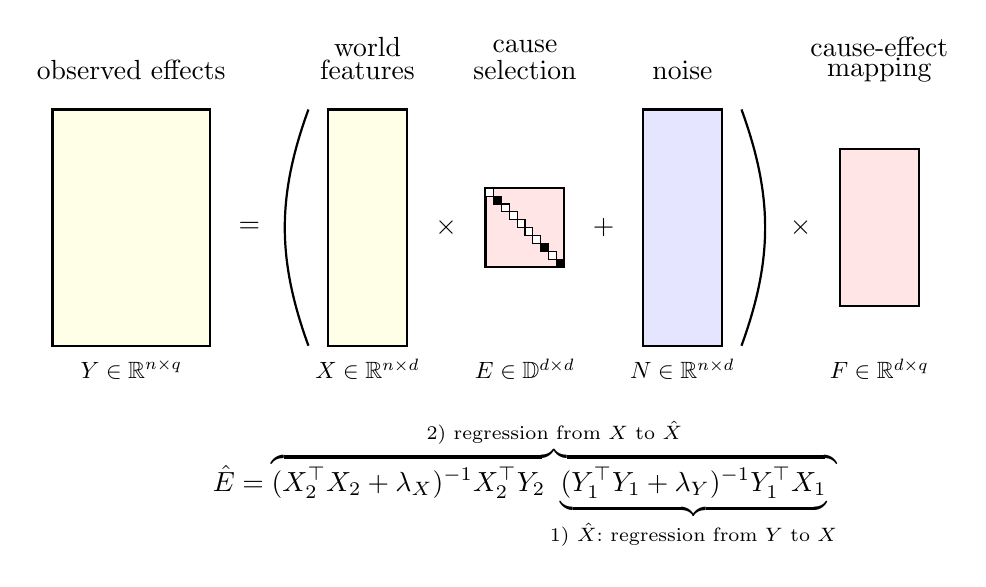
\begin{tikzpicture}
    \newcommand\posY{0}
    \newcommand\posX{3}
    \newcommand\posE{5}
    \newcommand\posN{7}
    \newcommand\posF{9.5}

    \node[thick, draw=black, minimum height=3cm, minimum width=2cm, fill=yellow!10] (Y) at (\posY, 0){};
    \node[] (eq) at (1.5, 0){$=$};
    \node[] (times) at (4, 0){$\times$};
    \node[thick, draw=black, minimum height=3cm, minimum width=1cm, fill=yellow!10] (X) at (\posX, 0){};
    \node[thick, draw=black, minimum height=1cm, minimum width=1cm, fill=red!10] (E) at (\posE, 0){};

    \draw[fill=white] (\posE - 0.5 + 0.0, 0.5 - 0.0) rectangle (\posE - 0.5 + 0.0 + 0.1, 0.5 - 0.0 - 0.1);
    \draw[fill=black] (\posE - 0.5 + 0.1, 0.5 - 0.1) rectangle (\posE - 0.5 + 0.1 + 0.1, 0.5 - 0.1 - 0.1);
    \draw[fill=white] (\posE - 0.5 + 0.2, 0.5 - 0.2) rectangle (\posE - 0.5 + 0.2 + 0.1, 0.5 - 0.2 - 0.1);
    \draw[fill=white] (\posE - 0.5 + 0.3, 0.5 - 0.3) rectangle (\posE - 0.5 + 0.3 + 0.1, 0.5 - 0.3 - 0.1);
    \draw[fill=white] (\posE - 0.5 + 0.4, 0.5 - 0.4) rectangle (\posE - 0.5 + 0.4 + 0.1, 0.5 - 0.4 - 0.1);
    \draw[fill=white] (\posE - 0.5 + 0.5, 0.5 - 0.5) rectangle (\posE - 0.5 + 0.5 + 0.1, 0.5 - 0.5 - 0.1);
    \draw[fill=white] (\posE - 0.5 + 0.6, 0.5 - 0.6) rectangle (\posE - 0.5 + 0.6 + 0.1, 0.5 - 0.6 - 0.1);
    \draw[fill=black] (\posE - 0.5 + 0.7, 0.5 - 0.7) rectangle (\posE - 0.5 + 0.7 + 0.1, 0.5 - 0.7 - 0.1);
    \draw[fill=white] (\posE - 0.5 + 0.8, 0.5 - 0.8) rectangle (\posE - 0.5 + 0.8 + 0.1, 0.5 - 0.8 - 0.1);
    \draw[fill=black] (\posE - 0.5 + 0.9, 0.5 - 0.9) rectangle (\posE - 0.5 + 0.9 + 0.1, 0.5 - 0.9 - 0.1);

    \node[] (plus) at (6, 0){$+$};
    \node[thick, draw=black, minimum height=3cm, minimum width=1cm, fill=blue!10] (N) at (\posN, 0){};
    \node[thick, draw=black, minimum height=2cm, minimum width=1cm, fill=red!10] (F) at (\posF, 0){};
    \draw [thick] (2.25, -1.5) to [round left paren ] (2.25, 1.5);
    \draw [thick] (7.75, -1.5) to [round right paren ] (7.75, 1.5);
    
    \node[] (times2) at (8.5, 0){$\times$};
    
    \node[] (annY) at (\posY, -1.8){\scalebox{0.85}{$Y \in \mathbb{R}^{n \times q}$}};
    \node[] (annX) at (\posX, -1.8){\scalebox{0.85}{$X \in \mathbb{R}^{n \times d}$}};
    \node[] (annE) at (\posE, -1.8){\scalebox{0.85}{$E \in \mathbb{D}^{d \times d}$}};
    \node[] (annN) at (\posN, -1.8){\scalebox{0.85}{$N \in \mathbb{R}^{n \times d}$}};
    \node[] (annF) at (\posF, -1.8){\scalebox{0.85}{$F \in \mathbb{R}^{d \times q}$}};

    \node[] (labY) at (\posY, 2){observed effects};
    \node[] (labX) at (\posX, 2.3){world};
    \node[] (labX) at (\posX, 2){features};
    \node[] (labE) at (\posE, 2.3){cause};
    \node[] (labE) at (\posE, 2){selection};
    \node[] (labN) at (\posN, 2){noise};
    \node[] (labF) at (\posF, 2.3){cause-effect};
    \node[] (labF) at (\posF, 2){mapping};
    
    \node[] (reg1) at (5,-3.25) {$\hat{E} = \overbrace{(X_2^\top X_2 + \lambda_X)^{-1} X_2^\top Y_2\underbrace{(Y_1^\top Y_1 + \lambda_Y)^{-1} Y_1^\top X_1}_{\text{1) } \hat{X} : \text{ regression from } Y \text{ to } X}}^{\text{2) regression from } X \text{ to } \hat{X}} $};
    \end{tikzpicture}
    \caption{Summary of our method blah blah blah}
    \label{fig:}
\end{figure}


\subsection{The method}

We are given two set of measurements over a sample of N individuals.
%
Y are ny multidimensional effects, and X are nx multidimensional possible causes.
%
We assume that only some features of X influence Y, so that $Y=f(EX,N)$, E being a binary diagonal, N some unknown noise, and f an unknown function.
%
We try to recover E, the active causal features.

Double regression consists in two steps.
%
First, we perform a least squares estimation of X from Y, that is we find $\hat G$ such that $\hat X=\hat G Y$ is the least square predictor of X.
%
This recovers an approximation of the causes of Y in X.
%
Then, we perform a least squares estimation of $\hat X$ from X, and determine $\hat H$ such that $\hat {\hat X}=\hat H X$ is the least square predictor of $\hat X$.
%
In matrix form, we have $\hat G=(Y'Y)^{-1} Y'X$, and
\begin{equation} \hat H=(X'X)^{-1} X'Y(Y'Y)^{-1} Y'X\end{equation}
Under good conditions (close to linear dependence between X and Y, and covariance matrices of X and Y well conditioned), this recovers a close approximation to E.

In practice, since the covariance matrices of Y and X might exhibit multicollinearity, we use regularisation in both matrix inversions.
%
This is done by using ridge regression, and determining at each step the regularisation parameter by cross validation.
%
In the above formula, this amounts to replacing $(X'X)^{-1}$ and $(Y'Y)^{-1}$ by $(X'X+\lambda)^{-1}$ and $(Y'Y+\mu)^{-1}$.
%
Also, to prevent spurious correlations between the two regressions (should they be performed on the same sample), our original sample is randomly split into two halves, and each step is performed over one of them, effectively decorrelating the two steps.
%
This is repeated over several (10) splits, and the resulting $\hat H$ are averaged.
%
This bagging compensates for the reduction in sample size caused by splitting.

Under our hypotheses (centred noise, E a binary diagonal) and even under heavy noise, $\hat H$ is close to diagonal.
%
Yet, because of regularisation which adds positive bias to small eigenvalues, and noise which attenuates large eigenvalues, $\hat H$ is in fact a scaled and noisy approximation to E.
%
To recover a binary diagonal, as our estimate of E, we extract the diagonal of $\hat H$ and select its large elements.
%
The diagonal matrix $\hat E$, having large elements of H as its unit diagonal coefficients (the rest being zero) is our estimate of E, the active features of X.

To select large elements of $\hat H$, the traditional approach in regression analysis consists in testing whether those coefficient differ from zero (or are larger from zero since we are only interested in large positive coefficients).
%
This is usually done via Student t-test of variants of it.
%
This will not work here, as double regression introduces, through two regularisations, a significant amount of positive bias on the diagonal, which depends in a complex manner on noise, dimensionality and conditioning of X and Y.
%
Instead, we treat feature extraction as a one dimensional binary clustering problem: classify n positive real values as "large" and "small" (under the hypothesis that they are not all small or all large).

This can be done by maximising the ratio of inter-group variance over total variance (ie minimising intra-group variance).
%
In a one dimensional two clusters setting, this amounts to sorting the data, and separating the p smallest from the n-p largest values so that inter group inertia is maximal.
%
If s and r are the average values of the two clusters, p and n-p their size and V the total variance of the sample, we are maximising the Sonquist and Morgan criterion $$K = {p (n-p) \over n} {(s-r)^2 \over V}$$ and selecting the p features corresponding to the largest values.
%
If diagonal elements of $\hat H$ are normally distributed, K follows a chi-square distribution with one degree of freedom.
%
At 95\% confidence level, a value of K superior to 3.84 makes our selection significant (for 99\% confidence, the corresponding value of K is 6.63) \citep{Kass_75}

This extract from $\hat H$ a binary diagonal $\hat E$.
%
To use double regression as a regression technique (to predict Y from X), we multiply X by $\hat E$ and perform a cross validated ridge regression of each feature of Y from $\hat E X$.

Summarizing, double regression is performed as follows:
\begin{enumerate}
\item Randomly split the data sample.
\item From the first half sample, using crossalidated ridge regression, find $\hat G$, the regularised least square regression of X from Y: $\hat G=(Y'Y)^{-1} Y'X$.
\item From the second half sample, calculate $\hat X = \hat G Y$, and find $\hat H$, the regularized least square regression of $\hat X$ from X: $\hat H=(X'X)^{-1} X'Y(Y'Y)^{-1} Y'X$.
\item Repeat steps 1 to 3 and average the results as $\hat H$.
\item Using the Sonquist and Morgan criterion, select the large diagonal elements of $\hat H$, set them to one and the rest of $\hat  H$ to zero.
\item Use the resulting matrix $\hat E$ as an estimator of E, the active features in the causal process
\item Alternatively, use $\hat E$ to predict Y from X, by performing a regularised least square regression of Y from $\hat E X$.
%

\end{enumerate}

\subsection{Asymptotic behaviour - linear case}
As discussed in the introduction, our problem can be formulated (up to a redifinition of the features of X) as $Y=f(MEX+N)$, with F an unknown function.
%
If F is linearm we can rewrite it as $Y = F(MEX + N)$, with X an (N, dx) matrix of possible causes, E a (dx,dx) binary diagonal matrix selecting active features of X.
%
M an unknown full rank (dz,dx) transformation of EX, N a (dz,N) homoscedastic noise matrix, F an unknown (possibly full rank) (dy,dz) transformation corresponding to the measuring apparatus, and Y a (dx,dy) matrix of measured effects.

Since N is centred, the first least square regression (X from Y), amounts to finding
\begin{equation}
\begin{aligned}
\min_G \left \| X-GY \right \|^2 &= \min_G \left \| X - GF(MEX+N)\right\|^2 \\
&{}= \min_G \left \| (I-GFME)X\right\| ^2 + \left \| GFN\right \| ^2\\
&{}\leq \min_G \left \| I-GFME\right\| ^2 \left \| X\right\| ^2 + k\left \| G\right \| ^2\\
\end{aligned}
\end{equation}
with k a positive constant which depends on the variance of FN.
%
This amounts to finding the minimal norm generalized inverse of FME, or its Moore-Penrose inverse $\hat  G= (FME)^{\dagger}$.

The second regression is from X to the predicted value of X in the above, or $\hat G Y$
\begin{equation}
\begin{aligned}
arg \min_H \left \| (FME)^{\dagger}Y - HX \right \|^2 &= arg \min_H \left \| (FME)^{\dagger}F(MEX+N) - HX \right \|^2 \\
&= arg \min_H \left \| ((FME)^{\dagger}(FME)-H)X \right \| ^2 + \left \| (FME)^{\dagger}FN \right \| ^2\\
&= arg \min_H \left \| ((FME)^{\dagger}(FME)-H)X \right \| ^2\\
&=(FME)^{\dagger}(FME)
\end{aligned}
\end{equation}
Thus, in the linear case, double regression retrieves $(FME)^{\dagger}(FME)$.

For any matrix A, $A^\dagger A$ is the orthogonal projector over $Img(A')$, and $I-A^\dagger A$ the orthogonal projector over $Ker(A)$.
%
In our case, $Ker(FME)\supseteq Ker(E)$.
%
If FM has full rank over the subspace spanned by the features selected by E (this is assumed for M and will happen for almost any random F), then $Ker(FME) = Ker(E)$,.
%
This means $I - \hat H$ is the projector over $Ker(E)$, the diagonal matrix that spans the unselected features, and $\hat H$ is the diagonal matrix corresponding to the selected features, that is E.
%
Under such hypotheses, $\hat H$ retrieves E, the features of X that have a causal influence on Y.
%
Since it is diagonal with eigenvalues well separated (0 and 1), it should do so in a fairly resilient way.

\subsection{Asymptotic behaviour - non linear case}

\subsection{Stability analysis}


\section{Related works}
\subsection{Double regression as a special case of canonical component analysis}
Formula (1) shows that double regression can be seen as a special case of canonical component analysis (CCA).
%
In CCA, we are given two matrixes X and Y (or size N,p and N,q) that describe different features measured on the same data sample, and characterise their proximity (that is, between the subspaces spanned by their columns) as the correlation between linear combinations of X and Y.

This is done by finding vectors $a$ and $b$ such that $Xa$ and $Yb$ display maximal correlation, or by maximising $a'X'Yb$ over unit-normed $a$ and $b$.
%
To find a, one calculates the eigenvectors of (1).
%
The largest one is the direction with maximal correlation, the second one the maximal correlation direction orthogonal to the first, and so on.
%
For each canonical dimension, the corresponding eigenvalue is the square of the cosine between the corresponding direction along X and the subspace spanned by Y.

If (1) is diagonal, for instance in the model presented above, the features of X are eigenvectors.
%
If all eigenvalues are either 0 or 1, since they correspond to the squared cosine of the angle between the corresponding feature and the subspace spanned by Y, all the features are either part of the Y subspace (eigenvalues of one) or orthogonal to it (for zero eigenvalues).
%
Thus, double regression amounts to CCA under the constraint that the subspaces spanned by X and Y are perpendicular, X is spanned by vectors of Y and vectors orthogonal to Y, and that the parallel and orthogonal components of X are spanned by disjoint sets of features of X.
%
The closer we are to this hypothesis, the closer the results of CCA and double regression will be.

There are differences between CCA and double regression.
%
First, since our objective is not to characterise the proximity between X and Y, but just to extract causal features, we can dispense with the last step of CCA (diagonalisation of (1)).
%
Second, since we operate in a noisy environment, we use regularisation, introducing bias in the correlation calculations.
%
Finally, whereas CCA wants to leverage all correlations between X and Y, we filter some of them, through splitting and bagging.
%
In other words, whereas we are working from the same formulae as CCA, we use them in different ways, for different purposes

\subsection{Related regression methods}
FC: discuss similar methods of regression, that can be used for feature extraction
And maybe have something about other causal discovery methods

\section{Experiments - simulated data}
Experiments on simulated data serve three goals: compare double regression with other known techniques (CCA, OLS, PLS...) both as regression and feature extraction methods, provide evidence for our claims on stability, invariance to environment, and behavior as a causal detector, and understand the strengths and limitations of double regression, and directions for future improvement.

The model used for simulation is $Y=f(snr MEX+N)$, with X a random (dx,N) matrix, E a square binary diagonal of dimension dx with the nc last elements equal to 1 (this means that of the dx features of X, only the nc last have some influence on Y), M and N (dz,dx) and (dz,N) random matrices, and f a function from $\mathbb{R}^{dz}$ to $\mathbb{R}^{dy}$, that can be linear or non linear.
%
In the linear case, the model becomes $Y=F(MEX+N)$, with F a (dy,dz) matrix.
%
In the non linear case, F becomes $FSH$ where F and H are matrices of dimensions (dz,dz) and (dy,dz), and S a vector of dz sigmoid transformations.
%
Finally, $snr$ is a real number measuring the amount of noise.

Our simulation therefore depends upon 6 free parameters : 
\begin{itemize}
\item dx : number of features of X
\item nc: number of active features (in EX)
\item dz: number of noise features
\item snr: signal to noise ratio
\item dy: number of features in Y
\item N: size of sample
\end{itemize}

Random matrices X, M, N, H and F are populated with centred gaussian random coefficients with unit variance, divided by $ \surd n$ where n is the smallest dimension of the matrix.
%
Since a random square matrix with unit gaussian coefficients of dimension n has eigenvalues between $ \surd n $ and $\surd n $, such  scaling allows for meaningful comparisons when dimensions dx, dy and dz vary.

FC: insert comment about scaling sigmoids, and maybe something about uniform coeffs

We evaluate the performance of double regression in two different roles : as a feature extractor recovering E, and as a regression method, predicting Y from X over a test sample.
%
For feature extraction, the quality of fit is the number of disagreements between our estimator and the diagonal of E (ie, their Hamming distance, which should be minimised).
%
For regression, we use a test set of N additional measurements, and calculate the R-squared ratio of variances (which should be maximised).
%
Performance indicators are calculated by averaging the results of several experiments.

\subsection{Feature extraction - linear case}
All other parameters being equal, the quality of feature extraction, measured as the discrepancy between features extracted by double regression ($\hat E$) and the diagonal of E, improves with signal to noise ratio.
%
The decrease is usually very steep until a Hamming distance under 2 is achieved.
%
Figure 1 presents a number of such curves for varying values of dx=dy=dz, nc=30 and N=1000.

Figure 1

The distance between $\hat E$ and E incorporates two different errors: false positives, where features not in E are extracted, and false negatives where features in E are not extracted.
%
For low values of the snr, and typical values of nc (much smaller than dx), false positives are high, but they fall faster as snr increases.
%
False negatives begin lower, but decrease more slowly (figure 2).
%
In other words, for each values of the parameters, one may determine a value of the signal to noise ratio, such that snr higher than this threshold allow for good feature extraction.
%
At this level, all the errors are false negatives.

Figure 2 

Working from a fixed sample of 1000, and 15 active features, and varying values of dx, dy, dz (from 50 to 200) and snr (from 0.2 to 1), we observe that, all other factors being equal, the quality of feature extraction and regression decrease when dx increases (X has more inactive features), dz increase (more noise dimensions) and snr decreases (less signal, more noise).
%
The dimensionality of Y plays a much smaller role, except for very small values of dy (less than 10).

For feature extraction, double regression either works very well (Hamming distance less than 2) or very badly, with a sharp change over small variations of the parameters.
%
The following graphs show the boundary between values of dx and dz that allow for features extractions (dx lower than boundary, or dz larger), for different values of dy (level curves on the graph), and different values of signal to noise ratio and number of active variables.

FC: add graphs here, see whether it is better to have nc fixed, or a proportion of dx, note : part of this can be moved to appendix if lack of space

For values of ...
%
in ..., an empirical formula can be provided.
%
Double regression allows for good feature extraction if : 

\subsection{Feature extraction - nonlinear case}


\subsection{Regression }
For regression, we want to understand how feature extraction helps predict Y from X.
%
To this effect, we compare four approaches to regression:
\begin{itemize}
\item standard ridge regression of Y from X, where no features are extracted this is our baseline
\item weighted ridge regression, of Y from $\hat H X$, where features of X are weighted according to the diagonal of $\hat H$
\item filtered ridge regression, of Y from $\hat E X$, where active features are first extracted (as above), and Y is predicted from the extracted features only  
\item perfect filtered (oracle) ridge regression of Y from EX, where E is supposed known 
\end{itemize}
Over a large set of parameters, we observe that filtered regression is on average better than weighted, which is on average better than standard regression.
%
This demonstrates that double regression can be used as a regression method, over the areas in parameter space where feature extraction performs well.

FC graphs go here

The quality of regression is independent from dy (except for very small values), increase with snr, decreases with dx, and increases with dz if it is larger than dx 
FC graphs go here

\subsection{Comparison with other methods}
Maxime territory

\subsection{Multiple environments}
In this section, we perform the same tests as in the previous one, but the test set is taken from a different distribution of X than the training set.
%
In practice, we test the same trained predictors of Y over test samples generated from a distribution of X with a different covariance.

The rationale behind such tests is that whereas double regression, being a feature extraction method, might not be as efficient as dedicated prediction tools, its focus on causal elements (and the removal of non causal features before carrying out regression) might cause it to be more resistant to changes in environments.

FC: ideally, we'd like to assess the multiple env performance of jrr, and compare it with others.
%
Are multiple environments limited to regression analyses? How should environments be generated (not just variance of X, I expect)?

\section{Experiments - real case}
Jean Remi and Maxime territory

\section{Conclusion}

\clearpage
\newpage

\bibliographystyle{abbrvnat}
\bibliography{paper}

\section{Appendices}

This should hold part of the tests, explanations on simulation, detailed results and stuff on meg data

\end{document}
